\section{Resultados e Discussão}
\label{sec:resultados}
%Tendo $n$ peixes no conjunto de testes para ser contados, os resultados a seguir apresentam a performace do método para a contagem de todos os peixe e em quadros que possuem $n$ peixes ou mais. Assim são apresentados os resultados para $n \geq \{1,2,4,6,8,10\}$ peixes, o acumulo de estágios e a utilização ou não do vetor de deslocamento no volume de entrada.


Nas subseções abaixo são demonstrados os resultados com detalhes condizente com os experimentos e as técnicas que geraram resultados relevantes.

\subsection{Resultados Quantitativos}
\label{subsec:ResultadosQ}
As Tabelas \ref{tab:resultadosGeral}, \ref{tab:resultadosEstagios} e \ref{tab:resultadosTemporal} mostram os resultados obtidos nos experimentos do método proposto após treinamentos de 100 épocas.
As tabelas apresentam a comparação dos resultados obtidos para diferentes variações de sigmas, número de estágios e o uso dos vetores de deslocamento como informação auxiliar na detecção dos objetos. 
Para uma avaliação adequada em desafios com vários peixes em um único quadro, nós reportamos as métricas em diversos cenários apresentados em cada coluna nas tabelas.
O primeiro considera o cálculo das métricas em todos os quadros do conjunto de teste (primeira coluna das tabelas).
Os demais cenários consideram somente quadros que contenham uma quantidade $i$ de peixes, e $i \geq {1,2,4,6,8,10}$.
%Os demais cenários consideram somente quadros com uma certa quantidade de peixes.
Por exemplo, a coluna $i \geq 10$ indica que somente foram considerados os quadros com 10 ou mais peixes no cálculo das métricas.
Portanto, o desafio imposto nesse cenário é muito maior quando comparado com quadros com poucos peixes.

%Para avaliar a quantidade de peixes contados em cada quadro, temos um comparativo referente a quantidade de peixes presentes em uma imagem. Desta forma os resultados apresentados se dão para os quadros que possuem uma quantidade $ i \geq  \{1,2,4,6,8,10\}$ de peixes.
%, o acumulo de estágios e a utilização ou não do vetor de deslocamento no volume de entrada
%Em negrito apresentam o melhor resultado.

%A contabilização dos quadros que contém a quantidade de peixes $\leq 6$, apresentam valores notoriamente inferiores para a função de erro $MAE$, em sua maioria os resultados são $\leq 1$ e muito próximos de 0. Por outro lado, a partir de 6 peixes na imagem a função alcança valores $\geq 1$. O teste com todos os quadros, por consequência todos os peixes $MAE = 0.116$ conforme a Tabela \ref{tab:resultadosGeral}.

%Em geral $R^2$ aponta valores inferiores quando a arquitetura não se adapta ao conjunto de dados, o melhor resultado obtido alcançou 94.1\%, que afirma o ajuste do modelo ao conjunto de dados. 
Conforme descrito da Seção \ref{sec:geracao_mapa}, a parâmetro $\sigma$ controla a largura dos picos que representa cada objeto no mapa de densidade.
Isto posto, a Tabela \ref{tab:resultadosGeral} apresenta os resultados dos experimentos realizados para uma variação do valor de $\sigma$.
Dessa forma, $\sigma = 0.7$ gera picos com um raio menor, enquanto $\sigma = 1.3$ gera picos com um raio maior. 
O número de estágio nesses experimentos foi fixado em $E = 4$.


%Ainda na Tabela \ref{tab:resultadosGeral}, temos um comparativo dos resultados obtidos, para cada valor de sigma, e a quantidade de peixes a serem contados em cada quadro. 
%Os valores exibidos apontam que quanto menor o valor de sigma, menor será os valores resultantes.
%Especialmente quando há uma quantidade significativa de peixes presentes é levado em consideração.


Analisando os resultados apresentados na Tabela \ref{tab:resultadosGeral}, podemos notar que o melhor resultado foi obtido para $\sigma = 1.1$, alcançando $F1 = 98\%$ e $MAE = 0.11$ de acertos e erros contabilizando todos os quadros.
Esse resultado é extremamente relevante pois o método proposta erra em média apenas 0.11 peixes por quadro.
Como esperado, quando a quantidade de peixes considerados por quadro aumenta, os valores de acertos diminuem.
Entretanto, mesmo quando somente quadros com 10 ou mais peixes são considerados, foram obtidos resultados relevantes com $F1 = 90\%$ e MAE = 1.71.
Para as variadas quantidade de peixes $\geq 1,2,4,6,8,10$ o melhor $\sigma$ obteve uma média de $F1 =  93\%$ de acertos.

%, valores presentes na Tabela \ref{tab:resultadosGeral}.

%dentre eles está a utilização dos 2 quadros processados, sendo 1 o quadro atual e 2 quadros anteriores para adquirir o deslocamento dos alevinos. Com a ciência da localização em 3 \textit{frames}, a função $F1$ aponta 96.8\% de acertos entre os Verdadeiros Positivos e os Falsos Positivos $\sigma_{max}$ = 3.0 e $\sigma_{min}$ = 1.5(Seção \ref{sec:geracao_mapa2}) conforme ilustrado na Tabela \ref{tab:resultados3} . O resultado que mais se destacou está na utilização de 2 quadros, com 98,4\% de exatidão da contagem no conjunto de testes para $\sigma_{max}$ = 2.0 e $\sigma_{min}$ = 1.5 (Tabela \ref{tab:resultados2}).

%\textbf{DISCUTIR OS RESULTADOS E COMPARAR DIFERENTES CNN, PROFUNDIDADE E COM A TESE }
%\newcolumntype{c}[1]{>{\centering\arraybackslash}c{#1}}



\begin{table}[h]
\small
\centering	
	\scalebox{0.63}{
	    \begin{tabular}{|p{1.2cm}|c|c|c|c|c|c|c|c|c|c|c|c|c|c|}
	%\begin{tabular}{|p{2cm}|p{1cm}|c|c|c|c|c|c|c|c|c|c|c|c|c|}
		\hline
		 \multirow{2}{\linewidth}{\centering \textbf{Sigma}} &
		 %\multicolumn{1}{|c|}{\textbf{Sigma}} & 
		 \multicolumn{2}{c|}{\textbf{Todos}} & 
		 \multicolumn{2}{c|}{$i \geq 1$} &
		 \multicolumn{2}{c|}{$i \geq 2$} &
		 \multicolumn{2}{c|}{$i \geq 4$} &
		 \multicolumn{2}{c|}{$i \geq 6$} &
		 \multicolumn{2}{c|}{$i \geq 8$} &
		 \multicolumn{2}{c|}{$i \geq 10$} 
		 \\
    	 \cline{2-15}
    	  & \textbf{MAE} & \textbf{F1} & 
          \textbf{MAE} & \textbf{F1} &
          \textbf{MAE} & \textbf{F1} &
          \textbf{MAE} & \textbf{F1} &
          \textbf{MAE} & \textbf{F1} &
          \textbf{MAE} & \textbf{F1} &
          \textbf{MAE} & \textbf{F1} 
         \\
         \hline
         \centering{$0.7$} & $0.343$ & $0.933$ & $0.561$ & $0.893$ & $0.823$ & $0.877$ & $1.372$ & $0.849$ & $2.958$ & $0.765$ & $3.133$ & $0.788$ & $3.071$ & $0.816$ \\ 
         \hline
         \centering{$0.8$} & $0.217$ & $0.960$ & $0.353$ & $0.938$ & $0.523$ & $0.926$ & $0.843$ & $0.915$ & $2.041$ & $0.852$ & $2.433$ & $0.842$ & $2.642$ & $0.843$
         \\
         \hline
         \centering{$0.9$} & $0.156$ & $0.975$ & $0.254$ & $0.960$ & $0.377$ & $0.952$ & $0.612$ & $0.945$ & $1.750$ & $0.878$ & $2.200$ & $0.858$ & $2.428$ & $0.857$
         \\
         \hline
         \centering{$1$} & $0.138$ & $0.978$ & $0.226$ & $0.965$ & $0.331$ & $0.959$ & $0.524$ & $0.954$ & $1.583$ & $0.891$ & $2.000$ & $0.872$ & $2.0$ & $0.885$
         \\
         \hline
         \centering{$\textbf{1.1}$} & $\textbf{0.116}$ & $\textbf{0.981}$ & $\textbf{0.189}$ & $\textbf{0.971}$ & $\textbf{0.274}$ & $\textbf{0.967}$ & $\textbf{0.431}$ & $\textbf{0.963}$ & $\textbf{1.354}$ & $\textbf{0.909}$ & $\textbf{1.766}$ & $\textbf{0.888}$ & $\textbf{1.714}$ & $\textbf{0.905}$
         \\
         \hline
         \centering{$1.2$} & $0.125$ & $0.980$ & $0.204$ & $0.969$ & $0.295$ & $0.965$ & $0.460$ & $0.961$ & $1.416$ & $0.904$ & $1.800$ & $0.886$ & $1.857$ & $0.895$
         \\
         \hline
         \centering{$1.3$} & $0.126$ & $0.982$ & $0.206$ & $0.972$ & $0.302$ & $0.965$ & $0.480$ & $0.959$ & $1.479$ & $0.900$ & $1.933$ & $0.877$ & $2.000$ & $0.886$
         \\
         \hline
	\end{tabular}}
	\caption{\label{tab:resultadosGeral} Resultados experimentais para a detecção dos alevinos com o método proposto. Comparação entre a variação dos $\sigma$ e estágios $E = 4$.}.
\end{table}

Outro parâmetro relevante do método proposto é a quantidade de estágios $E$.
Conforme a Seção \ref{sec:MetodoPrincipal}, os estágios podem ser concatenados para refinar as predições do mapa de densidade. Na Tabela \ref{tab:resultadosEstagios} temos os resultados para uma variação de $E$ em cada ramo da arquitetura proposta. 
%Para desmestificar a idéia de que quanto mais camadas convolucionais em uma rede, melhor será o seu desempenho.
%Os resultados apresentados são dos experimentos onde o(s) estágio(s) $e \in \{1,2,4,6\}$.
Os valores mostram que ao utilizar $E = 4$ estágios temos um resultado maior do que quando $E$ assume outros valores. 
As métricas para $E = 4$ estágios alcançaram o melhor resultado dentre os apresentados, tendo $98\%$ de acertos para a contabilização de todos os peixes.
Os resultados também mostram que usando $E < 4$ apresenta valores excelentes para a contagem de todos os peixes, mas quando a contagem acontece por meio da quantidade de peixes em cada quadro, o método mostrou uma queda na eficiência de contagem. 
Isso mostra que os estágios ajudam a refinar o mapa para a contagem dos objetos.

\begin{table}[h]
\small
\centering	
	\scalebox{0.62}{
	    \begin{tabular}{|p{1.6cm}|c|c|c|c|c|c|c|c|c|c|c|c|c|c|}
	%\begin{tabular}{|p{2cm}|p{1cm}|c|c|c|c|c|c|c|c|c|c|c|c|c|}
		\hline
		 \multirow{2}{\linewidth}{\centering \textbf{Estágios}} &
		 %\multicolumn{1}{|c|}{\textbf{Sigma}} & 
		 \multicolumn{2}{c|}{\textbf{Todos}} & 
		 \multicolumn{2}{c|}{$i \geq 1$} &
		 \multicolumn{2}{c|}{$i \geq 2$} &
		 \multicolumn{2}{c|}{$i \geq 4$} &
		 \multicolumn{2}{c|}{$i \geq 6$} &
		 \multicolumn{2}{c|}{$i \geq 8$} &
		 \multicolumn{2}{c|}{$i \geq 10$} 
		 \\
    	 \cline{2-15}
    	  & \textbf{MAE} & \textbf{F1} & 
          \textbf{MAE} & \textbf{F1} &
          \textbf{MAE} & \textbf{F1} &
          \textbf{MAE} & \textbf{F1} &
          \textbf{MAE} & \textbf{F1} &
          \textbf{MAE} & \textbf{F1} &
          \textbf{MAE} & \textbf{F1} 
         \\
         \hline
         \centering{$1$} & $0.227$ & $0.955$ & $0.368$ & $0.931$ & $0.483$ & $0.928$ & $0.598$ & $0.939$ & $1.333$ & $0.902$ & $1.700$ & $0.880$ & $1.785$ & $0.899$ 
         \\
         \hline
         \centering{$2$} & $0.140$ & $0.976$ & $0.227$ & $0.964$ & $0.333$ & $0.959$ & $0.524$ & $0.952$ & $1.520$ & $0.890$ & $1.900$ & $0.871$ & $2.071$ & $0.881$ 
         \\
         \hline
         \centering{$\textbf{4}$} & $\textbf{0.116}$ & $\textbf{0.981}$ & $\textbf{0.189}$ & $\textbf{0.971}$ & $\textbf{0.274}$ & $\textbf{0.967}$ & $\textbf{0.431}$ & $\textbf{0.963}$ & $\textbf{1.354}$ & $\textbf{0.909}$ & $\textbf{1.766}$ & $\textbf{0.888}$ & $\textbf{1.714}$ & $\textbf{0.905}$ 
         \\
         \hline
         \centering{$6$} & $0.122$ & $0.980$ & $0.198$ & $0.969$ & $0.288$ & $0.965$ & $0.451$ & $0.961$ & $1.395$ & $0.905$ & $1.800$ & $0.886$ & $1.714$ & $0.904$ 
         \\
         \hline
	\end{tabular}}
	\caption{\label{tab:resultadosEstagios} Resultados experimentais para a detecção dos alevinos com o método proposto. Comparação entre a variação na quantidade de estágios E usando $\sigma = 1.1$}.
\end{table}

Após o modelo proposto apresentar o melhor resultado utilizando $E = 4$ estágios e $\sigma = 1.1$, os resultados da Tabela \ref{tab:resultadosTemporal} mostra a comparação do uso ou não do ramo que estima os vetores de deslocamento temporal conforme a Seção \ref{sec:Images}.
Apesar dos valores similares, o resultado se destaca quando o ramo que estima os vetores de deslocamento é utilizado.
Isso corrobora que a inclusão de informação mesmo que indireta da localização do objeto anteriormente melhora os resultados.

\begin{table}[h]
\small
\centering	
	\scalebox{0.60}{
	    \begin{tabular}{|p{1.8cm}|c|c|c|c|c|c|c|c|c|c|c|c|c|c|}
	%\begin{tabular}{|p{2cm}|p{1cm}|c|c|c|c|c|c|c|c|c|c|c|c|c|}
		\hline
		 \multirow{2}{\linewidth}{\centering \textbf{Temporal}} &
		 %\multicolumn{1}{|c|}{\textbf{Sigma}} & 
		 \multicolumn{2}{c|}{\textbf{Todos}} & 
		 \multicolumn{2}{c|}{$i \geq 1$} &
		 \multicolumn{2}{c|}{$i \geq 2$} &
		 \multicolumn{2}{c|}{$i \geq 4$} &
		 \multicolumn{2}{c|}{$i \geq 6$} &
		 \multicolumn{2}{c|}{$i \geq 8$} &
		 \multicolumn{2}{c|}{$i \geq 10$} 
		 \\
    	 \cline{2-15}
    	  & \textbf{MAE} & \textbf{F1} & 
          \textbf{MAE} & \textbf{F1} &
          \textbf{MAE} & \textbf{F1} &
          \textbf{MAE} & \textbf{F1} &
          \textbf{MAE} & \textbf{F1} &
          \textbf{MAE} & \textbf{F1} &
          \textbf{MAE} & \textbf{F1} 
         \\
         \hline
         \centering{\textbf{Sim}} & $\textbf{0.116}$ & $\textbf{0.981}$ & $\textbf{0.189}$ & $\textbf{0.971}$ & $\textbf{0.274}$ & $\textbf{0.967}$ & $\textbf{0.431}$ & $\textbf{0.963}$ & $\textbf{1.354}$ & $\textbf{0.909}$ & $\textbf{1.766}$ & $\textbf{0.888}$ & $\textbf{1.714}$ & $\textbf{0.905}$ 
         \\
         \hline
         \centering{Não} & $0.138$ & $0.978$ & $0.227$ & $0.964$ & $0.328$ & $0.959$ & $0.534$ & $0.949$ & $1.500$ & $0.897$ & $1.866$ & $0.882$ & $1.928$ & $0.891$ 
         \\
         \hline
	\end{tabular}}
	\caption{\label{tab:resultadosTemporal} Resultados experimentais para a detecção dos alevinos com o método proposto, $E = 4$ estágios, e $\sigma = 1.1$. Comparação do método com e sem os vetores de deslocamento dos peixes, denominado temporal}.
\end{table}


%O OKS conforme já citado na seções anteriores calcula a relação entre os pontos apontados nas \textit{anotações} e os pontos \textit{preditos}, sendo assim seu valor aponta o quanto a predição está correta quantitativamente, temos 82.9\% de exatidão das predições.


%\begin{table}[h]
%	\centering	
%	\begin{tabular}{|p{2cm}|p{1cm}|c|c|c|c|c|c|c|}
%		\hline
%		 \multirow{2}{\linewidth}{\centering Quadro(s) ($T$)} &
%		 \multirow{2}{\linewidth}{\centering $\sigma_{min}$} &
%		 \multicolumn{4}{c|}{\textbf{Métricas de Erro}} & \multicolumn{3}{c|}{\textbf{Métrica F1}} \\
%    	\cline{3-9}
%    	  & &\textbf{MAE} & \textbf{MSE} & \textbf{NRMSE} & {$\textbf{R}^{2}$} &\textbf{Precisão} & \textbf{Revocação} & \textbf{F1} \\
%    	%\cline{3-9}
%		\hline
%		
%		 \multirow{3}{\linewidth}{\centering \textbf{1}} & \centering{$0.5$} & $0.337$ & $0.523$ & $0.889$ & $0$  & $0.967$ & $0.900$ & $0.926$\\
%		 & \centering{$1.5$} & $0.131$ & $0.170$ & $0$& $0.963$ & $0.993$ & $0.972$ & $0.981$\\
%		 & \centering{$2.0$} & $0.142$ & $0.198$ & $0$ & $0.957$ & $0.997$ & $0.974$ & $0.983$\\
%		\hline
%		
%		\multirow{3}{\linewidth}{\centering \textbf{2}} & \centering{$0.5$} & $0.321$ & $0.521$ & $0$ & $0.889$  & $0.964$ & $0.903$ & $0.927$\\
%		 & \centering{$\textbf{1.5}$} & $\textbf{0.119}$ & $\textbf{0.153}$ & $\textbf{0}$ & $\textbf{0.967}$ & $\textbf{0.995}$ & $\textbf{0.978}$ & $\textbf{0.984}$\\
%		 & \centering{$2.0$} & $0.126$ & $0.166$ & $0$ & $0.964$ & $0.995$ & $0.978$ & $0.984$\\
%		\hline
%		
%		\multirow{3}{\linewidth}{\centering \textbf{3}} & \centering{$0.5$} & $0.331$ & $0.559$ & $0$ & $0.881$  & $0.966$ & $0.904$ & $0.928$\\
%		 & \centering{$1.5$} & $0.212$ & $0.322$ & $0$& $0.931$ & $0.989$ & $0.954$ & $0.967$\\
%		 & \centering{$2.0$} & $0.239$ & $0.366$ & $0$ & $0.922$ & $0.988$ & $0.949$ & $0.964$\\
%		\hline%

%	\end{tabular}
%	\caption{\label{tab:resultados2} Resultados experimentais para a detecção dos alevinos com a arquitetura VGGNet + estágios de refinamentos. Comparação entre a quantidade de quadros processados para $\sigma_{max} = 2.0$ e estágios $E = 4$.}.
%\end{table}


%O resultado para a métrica de erro MAE impulsiona positivamente o modelo para a contagem de alevinos. A Tabela \ref{tab:comparation} contém quantitativamente os resultados da métrica de erro MAE, apontado na dissertação de mestrado de \cite{Junior2019UFMS}, como o melhor resultado apresentado pelo seu método. Os resultados da proposta deste texto também estão presentes para a mesma métrica. A comparação numérica dos valores indica uma acentuação favorável para a proposta desta dissertação, tendo valores muito próximo de $0$. Os dois resultados são para a contagem de alevinos, porém \cite{Junior2019UFMS} apresenta técnicas divergentes da deste texto, que por sua vez, recebe um ponto para indicar a presença de um alevino (vide Seção \ref{sec:relatedWork}).
%A dissertação de mestrado de \cite{Junior2019UFMS}, apresenta uma estimativa da massa dos alevinos, são comparados maneiras


%\begin{table}[htb]
%	\centering	
%	\begin{tabular}{|c|c|}
%		\hline
%		\textbf{Abordagem} & \textbf{MAE} \\
%		\hline
%		Proposta & $0.12$ \\
%		\hline
%		Tese Oliveira J. & $5.99$  \\
%		\hline
%	\end{tabular}
 %   \caption{\label{tab:comparation} Resultados experimentais para a identificação dos alevinos com a arquitetura VGGNet comparada com o trabalho de \cite{Junior2019UFMS}}.
%\end{table}

\subsection{Resultados Qualitativos}

A Figura \ref{fig:resultadosQuali} ilustra como o mapa de densidade representa a presença de um alevino na imagem. Cada pico apontado no \textit{Heatmap} consiste na presença de um alevino.

   \begin{figure}[htb]
	\noindent\makebox[\textwidth]{%
		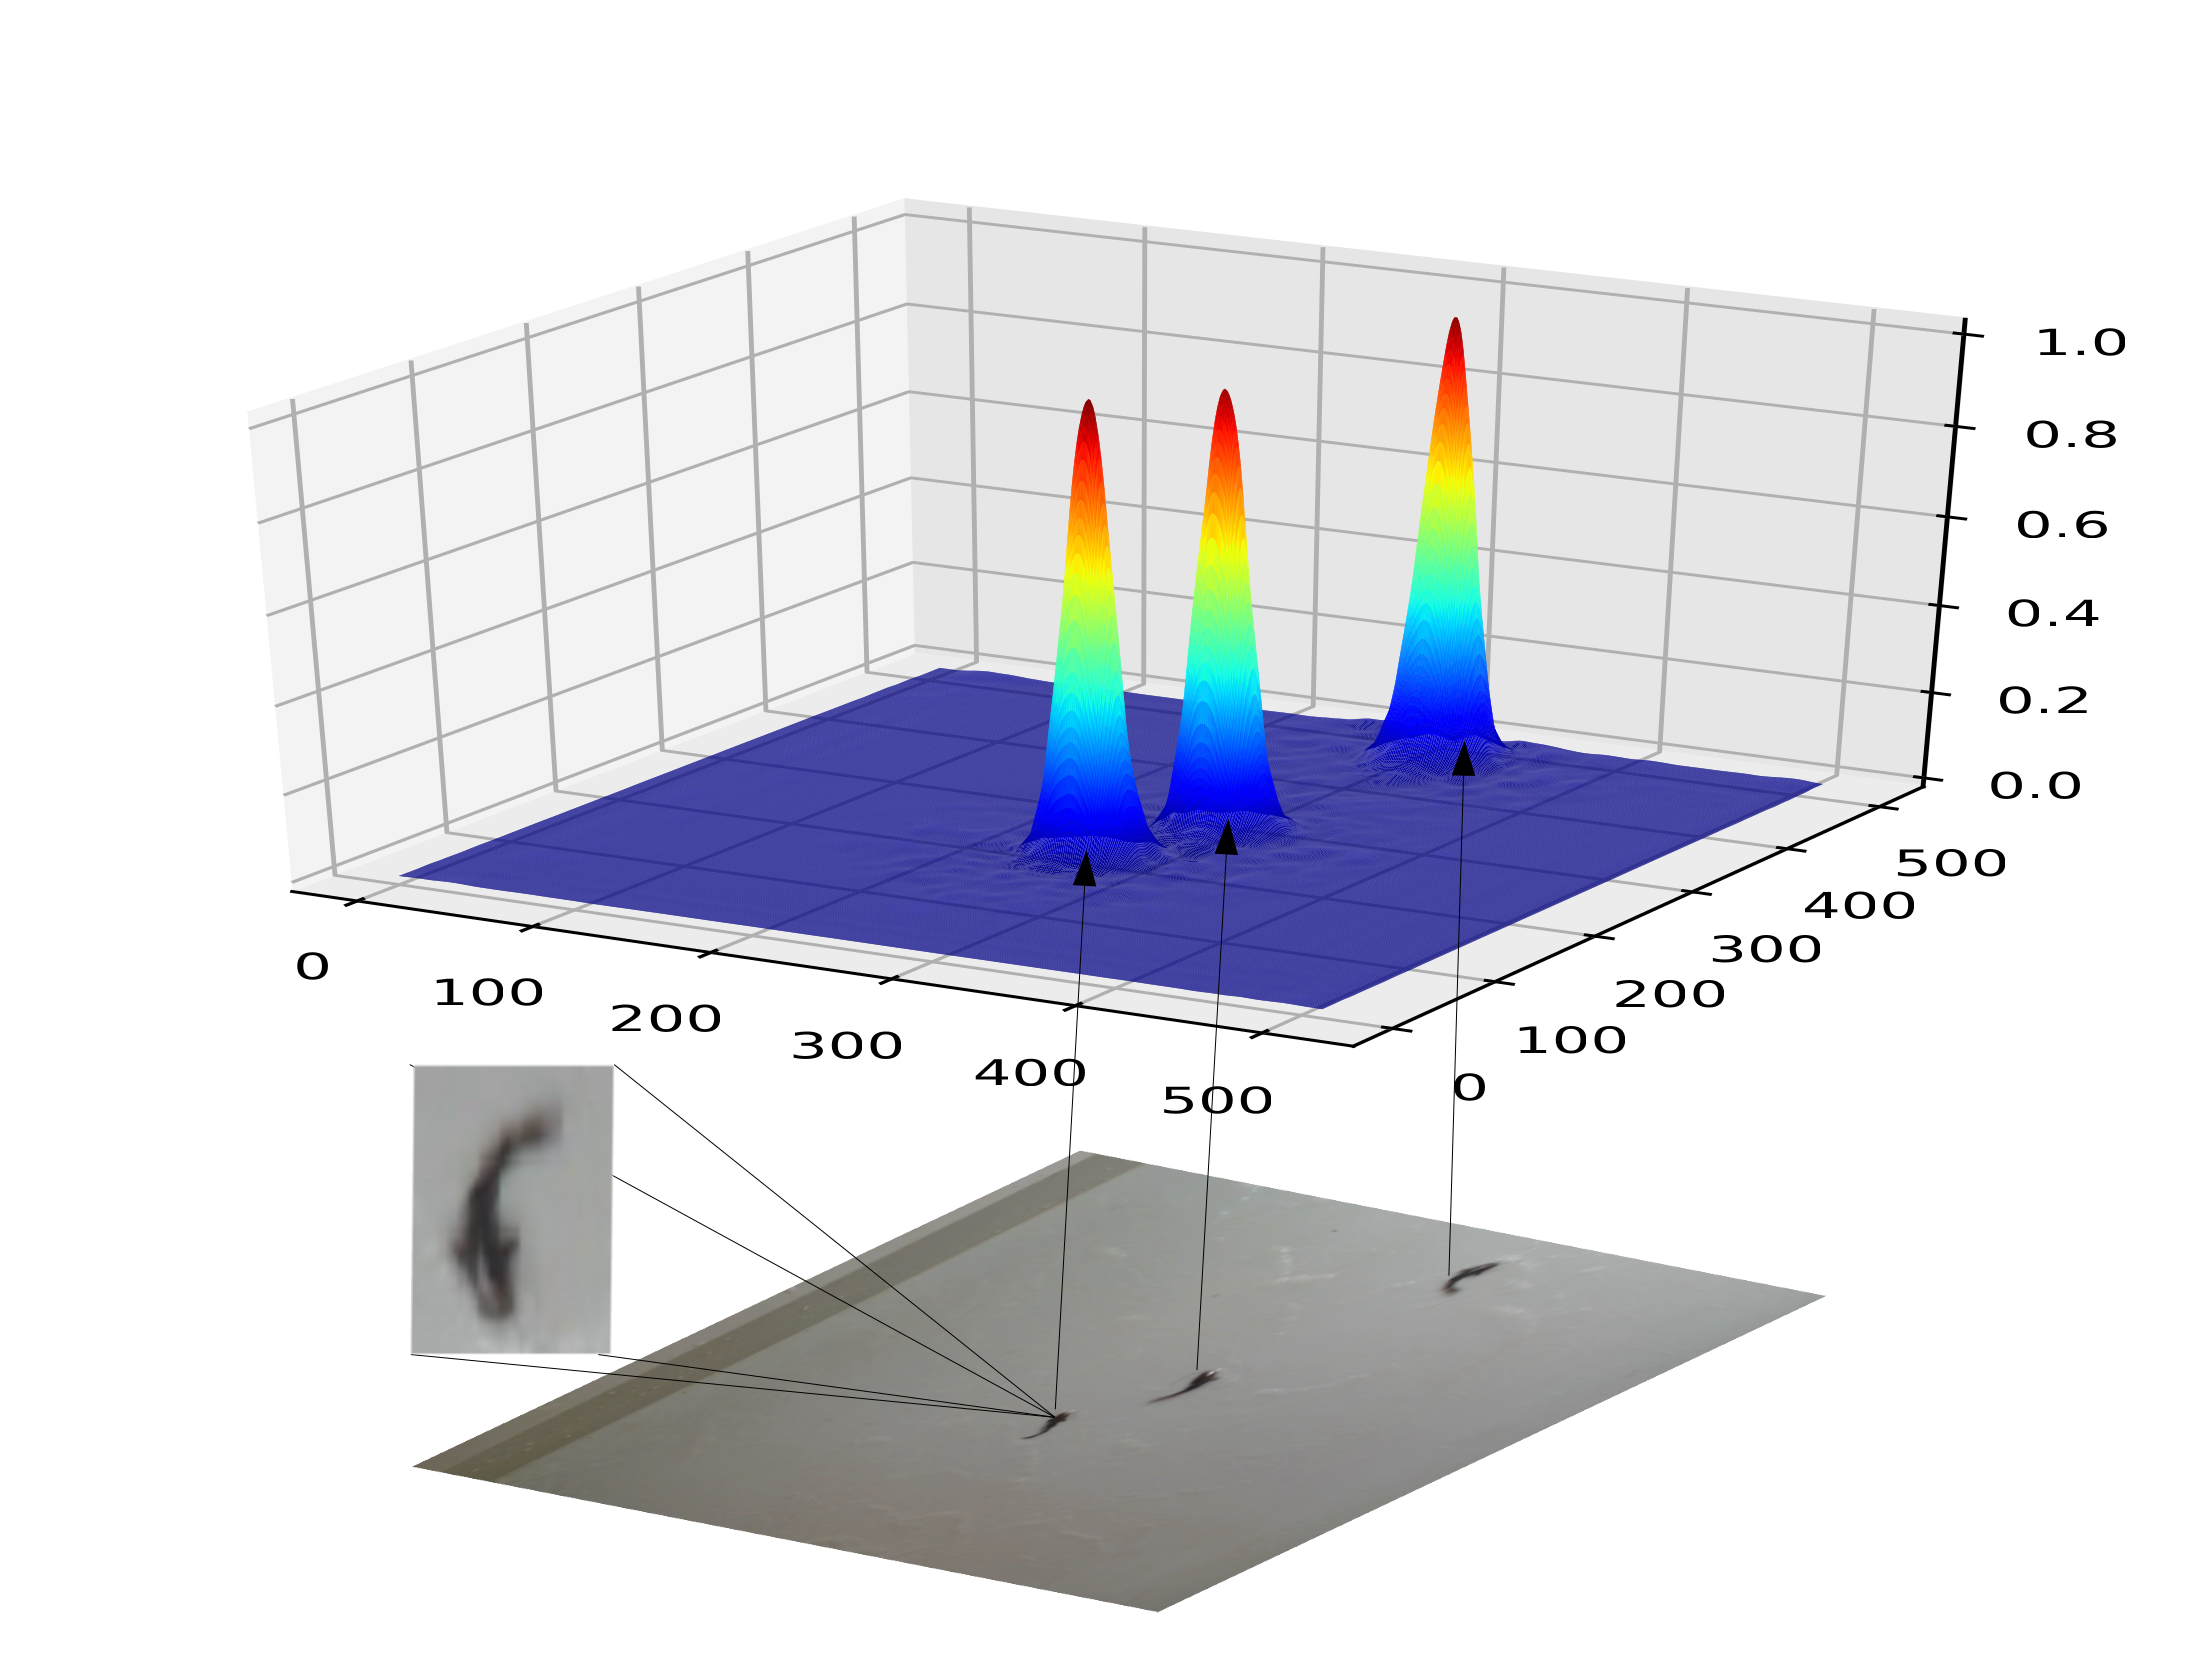
\includegraphics[width=0.9\textwidth]{image/VID06_frame000147.png}}
	\caption{Ilustração do \textit{Heatmap} obtido do \textit{frame} 147 do vídeo número 6, predito pelo modelo treinado por 100 épocas.}
	\label{heatmap}
    \end{figure}

Podemos observar nas imagens da Figura \ref{fig:resultadosQuali} o quadro original, o mapa de densidade, as detecções e a avaliação da métrica \textit{F1} e a estimativa dos vetores de deslocamento.
Todos os peixes presente no quadro foram detectados e os vetores foram estimatidos para as posições anteriores. Neste caso em específico temos dois peixes próximos que foram detectados e contabilizados individualmente.
%Na maioria das vezes os peixes não muito próximos são facilmente detectados.

Haja vista a Seção \ref{subsec:ResultadosQ} os quadros onde a quantidade de alevinos é $\leq 6$, os alevinos são facilmente detectados. Quando a presença de peixes é $\geq 6$ a CNN detecta os alevinos em sua grande maioria, mas existe aqueles que por algum motivo tiveram uma deformação em sua forma na imagem. O movimento realizado pelo peixe diz muito sobre a sua forma.

\begin{figure}[!hbt]
	\centering
	\subfloat[Imagem Original]{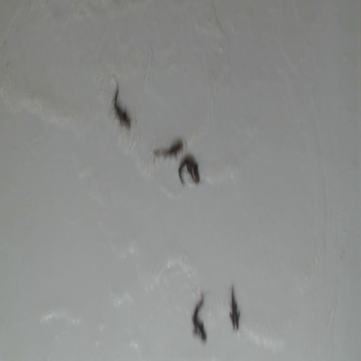
\includegraphics[width=0.4\textwidth]{image/ResultadosQ/VID09_frame000039.png}}\vspace{0.9cm}	
	\subfloat[Mapa de densidade]{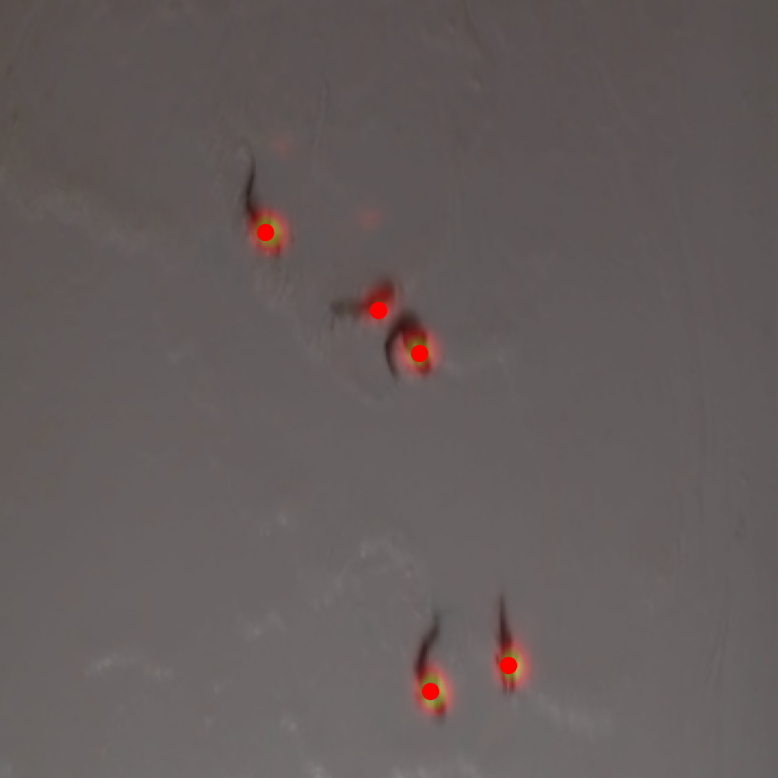
\includegraphics[width=0.4\textwidth]{image/ResultadosQ/VID09_frame000039_points_.png}}\vspace{0.2cm}	
	\subfloat[Predições]{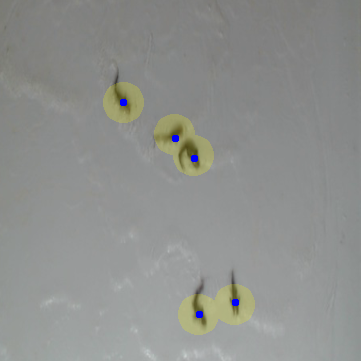
\includegraphics[width=0.4\textwidth]{image/ResultadosQ/VID09_frame000039_points.png}}\vspace{0.2cm}
	\subfloat[Estimativa dos Vetores de Deslocamento]{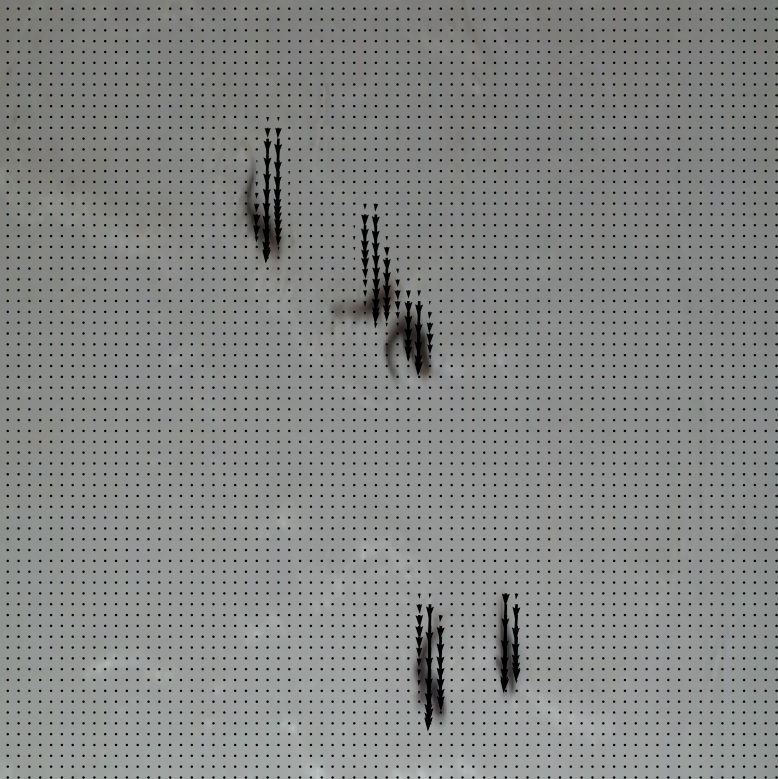
\includegraphics[width=0.4\textwidth]{image/ResultadosQ/VID09_frame000039_vectors.png}}%\vspace{0.2cm}

	\caption{\label{fig:resultadosQuali} Exemplos dos resultados visuais obtidos para o quadro 30 do vídeo 09. A Figura (a) mostra a imagem original, (b) o mapa de densidade, (c) as predições e (d) a estimação dos vetores.
	%As subfiguras (a,b,c) possui as imagens originais, (d,e,f) contém os \textit{heatmaps} obtidos e (g,h,i) os resultados da Métrica F1. 
	%\textbf{TROCAR por IMAGENS da pasta "melhoresResultadosVisuais"}
	}
\end{figure}

Um dos problemas da abordagem proposta esta na detecção correta do alevino quando parte do seu corpo está oclusa na imagem. Isso acontece, pois uma das características da CNN é buscar identificar o alevino considerando uma distribuição de probabilidade de um alevino estar em um pixel. Dessa forma, para que a CNN consiga predizer um alevino, boa parte do formato dele deve aparecer na imagem, para que uma resposta alta a esse padrão seja encontrada. 


Nas imagens presentes na Figura \ref{fig:resultadosJuntos} temos um quadro onde existem três alevinos, porém os dois mais próximos, foram contabilizados apenas como um. Um alevino encontra-se extremamente próximo ao outro, impossibilitando de serem distinguidos a olho nu.
Em alguns quadros na sequência temos que os dois peixes chegam a se separar, porém existem casos em que dois alevinos se movem uniformemente. Essa aproximação confundi a estimativa de vetores, que estima um número de vetores deslocamento diferente.

\begin{figure}[!htb]
	\centering
	\subfloat[Imagem Original]{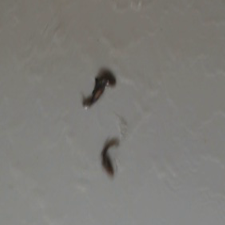
\includegraphics[width=0.35\textwidth]{image/ResultadosQ2/VID11_frame000217.png}}\vspace{0.9cm}	
	\subfloat[\textit{Ground Truth}]{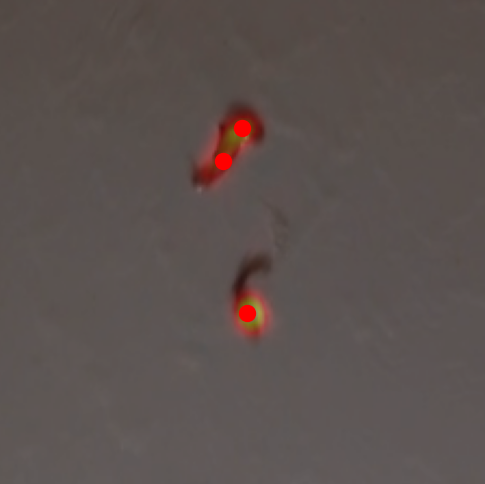
\includegraphics[width=0.35\textwidth]{image/ResultadosQ2/VID11_frame000217_points_gt_.png}}\vspace{0.2cm}	
	\subfloat[Predições]{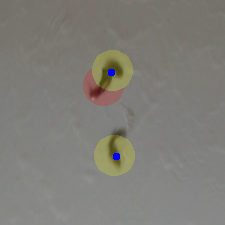
\includegraphics[width=0.35\textwidth]{image/ResultadosQ2/VID11_frame000217_points.png}}\vspace{0.2cm}
	\subfloat[Estimativa dos Vetores de Deslocamento]{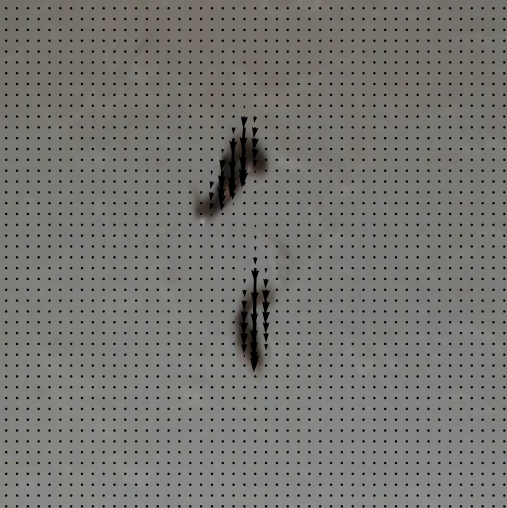
\includegraphics[width=0.35\textwidth]{image/ResultadosQ2/VID11_frame000217_vectors.png}}%\vspace{0.2cm}

	\caption{\label{fig:resultadosJuntos} Exemplos dos resultados visuais obtidos para o quadro 270 do vídeo 11. A Figura (a) nos mostra a imagem original, (b) o mapa de densidade, (c) as predições e (d) a estimação dos vetores.
	%As subfiguras (a,b,c) possui as imagens originais, (d,e,f) contém os \textit{heatmaps} obtidos e (g,h,i) os resultados da Métrica F1. 
	%\textbf{TROCAR por IMAGENS da pasta "melhoresResultadosVisuais"}
	}
	
\end{figure}

%Podemos observar nas imagens \ref{fig:resultadosQuali} que alevinos rigorosamente próximos conseguem ser detectados individualmente. Em especifico na sub figura (a) e (d) temos um exemplos de um frame que contém dois alevinos distantes são identificados corretamente, na sub figura (b) e temos $10$ alevinos presentes nas imagens porém os peixes muito próximos, quase que imperceptível a olho nu, são confundidos pelo método que aponta apenas a presença de $8$ alevinos presentes (figura (e)). A região dos alevinos próximos é apontada como um alevino apenas, isso acontece devido a extrema proximidade que se mantém também nos \textit{frames} anteriores. Nas figuras (c) e (f) nos mostra que os alevinos próximos que mantém uma certa distância, assim como nos quadros anteriores são corretamente detectados pelo método.

%As imagens (b) e (e) da Figura \ref{fig:resultadosQuali} mostra os principais desafios enfrentados pela abordagem proposta. 

Por outro lado, outro grande desafio é detectar corretamente o formato do alevino na imagem. Podemos observar que quase sempre por conta da colisão entre eles os alevinos formam um padrão disforme ao usual.
Apesar desses desafios, o método proposto é capaz de detectar corretamente a grande maioria dos alevinos.
%dois volumes centrais na imagem ao invés de um, podemos ver que a rede pode em alguns casos, predizendo que existem dois alevinos nessas posições. Porém, esse erro tende a diminuir, uma vez que aumentamos o número de imagens de treinamento, pois a rede neural convolucional começa aprender os diferentes formatos que os alevinos podem aparecer nas imagens.

%Nas subfiguras (g,h e i) da Figura \ref{fig:resultadosQuali} temos o resultados obtido pela Métrica F1. Os pontos azuis são as detecções, o círculo amarelo em torno dos peixes são os verdadeiros positivos, ou seja, que foram detectados corretamente. Os círculos vermelhos são os Falsos Negativos, onde há a presença de um peixe porém a arquitetura não o identificou.

%\textbf{DISCUTIR OS RESULTADOS VISUAIS DA NOSSA ABORDAGEM -> na pasta "melhoresResultadosVisuais" tem as imagens onde a técnica detectou corretamente os alevino -> só escolher as 6 melhores e explicar pq ela teve bom resultado..EX: mesmo alevinos grudados, a técnica detectou bem, pois considera o heatmap, etc, etc ...}
